% !iTeXMac(input): POH.tex
\chapter{WEIGHT \& BALANCE}
\vspace{\minitocspacebefore}
\minitoc
%\mtcskip
%\minilof
\cleardoublepage

\section{INTRODUCTION}
This section describes the procedure for establishing the basic empty weight and moment of 
the aircraft.  Sample forms are provided for reference.  Procedures for calculating the 
weight and moment for various operations are also provided.  

\section{AIRCRAFT WEIGHING PROCEDURES}
\begin{enumerate}
  \item Preparation:
    \begin{enumerate}
      \item Inflate tires to recommended operating pressures.
      \item Drain all fuel from the fuel tanks.
      \item Ensure the oil sump is filled to 8 US quarts.
      \item Remove all items from forward and aft baggage area and cockpit pockets.
      \item Raise flaps to the fully retracted position.
      \item Place all control surfaces in the neutral position.
    \end{enumerate}
  \item Levelling:
    \begin{enumerate}
      \item Place scales under each wheel (minimum capacity, 600 lb for main gear, 200 lb for tail wheel).
      \item Place shims under main wheels as necessary to level aircraft laterally.
      \item Raise tail wheel with support until a level on the canopy rail indicates level.
      \suspend{enumerate}
  
   \resume{enumerate}
   \item Close and lock the canopy.
    \end{enumerate}
  \item Weighing:
  \label{weighing}
    \begin{enumerate}
      \item With the aircraft level, record weight shown on each scale.  Deduct the tare weight from each reading.
    \end{enumerate}
  \item Measuring:
  \label{measuring}
    \begin{enumerate}
      \item Drop a plumb bob from the wing leading edge behind each main gear and mark the floor.  Measure 70 inches
forward of this line and mark the floor for the location of the datum.
      \item Measure the horizontal distance from the datum (parallel to the aircraft centre line) to each main wheel
centre.
      \item Measure the horizontal distance (along the aircraft centre line) from the datum to the centre
of the tail wheel axle.
    \end{enumerate}
  \item Using weights from item \ref{weighing} and measurements from item \ref{measuring}, the aircraft weight and CG
can be determined.\label{calc-wb}
  \item Basic Empty Weight may be determined by completing Figure \ref{WB-SampleChart}.
  \end{enumerate}

\begin{figure}
\addcontentsline{toc}{section}{Figure \ref{WB-SampleChart} Sample Aircraft Weighing Record}
\begin{center}
\begin{perfhdr}SAMPLE AIRCRAFT WEIGHING RECORD
  \end{perfhdr}
\settowidth{\colOne}{Right Wheel}
\settowidth{\colTwo}{Distance}
\settowidth{\colThree}{Reading}
\settowidth{\colFour}{Tare}
\settowidth{\colFive}{Weight}
\settowidth{\colSix}{(Moment/1000)}

\begin{overpic}[scale=.7]{../Diagrams/WB-SideView}
  \put(42.3,18.1){CG}
  \put(6,16){70"}
  \put(12,7){DL \& DR}
  \put(70,3){DT}
  \put(19,30.5){X}
  \put(-5,15){\rotatebox{90}{DATUM}}
  % cgspot is not working with dvipdfmx
  % \put(39.2,17.7){
\includegraphics[scale=0.08]{../Diagrams/cgspot}}
  \put(39.2,17.7){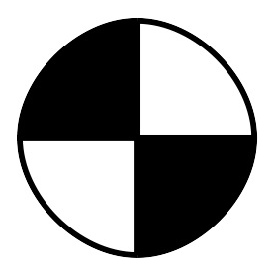
\includegraphics[scale=0.08]{../Diagrams/cgspot2}}
  \end{overpic}  

\vspace{0.2in}
\begin{tabular}{|l|c|c|c|c|c|}
\hline
&\multirow{4}{\colTwo}{\centering Arm (in)}&\multirow{4}{\colThree}{\centering Scale
Reading (lb)}&\multirow{4}{\colFour}{\centering Tare (lb)}&\multirow{4}{\colFive}{\centering Net Weight (lb)}&

\multicolumn{1}{c|}{Moment/1000}\\
\multicolumn{1}{|c|}{Scale}&&&&&\multicolumn{1}{c|}{(Arm x Net}\\
\multicolumn{1}{|c|}{Position}&&&&&\multicolumn{1}{c|}{Weight/1000)}\\
&&&&&\multicolumn{1}{c|}{(lb-in)}\\
\hline
\hline
Left Wheel&\multicolumn{1}{l|}{DL=\hspace*{.7in}}&&&\multicolumn{1}{l|}{L=}&\\
\hline
Right Wheel&\multicolumn{1}{l|}{DR=}&&&\multicolumn{1}{l|}{R=}&\\
\hline
Tail Wheel&\multicolumn{1}{l|}{DT=}&&&\multicolumn{1}{l|}{T=}&\\
%\whline
\hline
\hline
\multicolumn{4}{|l|}{Sum of Net Weights and Moments}&W=\hspace*{.7in}&M=\hspace*{1in}\\
\hline
\end{tabular}\\
\vspace{.2in}
\begin{tabular}{lcr}
$\mathrm{CG(X)=ARM=\frac{M}{W}}$&\hspace{1in}&CG(X)=\makebox[.75in]{\hrulefill} in
\end{tabular}
\vspace{0.2in}
\settowidth{\colOne}{Aircraft Weight (From Item \ref{calc-wb}, page \pageref{calc-wb})}
\settowidth{\colTwo}{Weight}
\settowidth{\colThree}{CG Arm}
\begin{tabular}{|l|c|c|c|}
\hline
\multirow{2}{\colOne}{\centering Item}&\multirow{2}{\colTwo}{\centering Weight (lb)}&\multirow{2}{\colThree}{\centering CG Arm (in)}&Moment/1000\\
&&&(lb-in)\\
\hline
\hline
Aircraft Weight (From Item \ref{calc-wb}, page \pageref{calc-wb})&&&\\
% \hline
% Add Oil: (\textcolor{red}{XX} Qts at 7.5 lbs/Gal)&&\textcolor{red}{XX} in&\\
\hline
Add Unusable Fuel: (0.2 USG at 6.01 lbs/Gal)&&\textcolor{red}{XX} in&\\
\hline
Equipment Changes&&&\\
%\whline
\hline
\hline
Aircraft Basic Empty Weight&&&\\
\hline
\end{tabular}
\end{center}

\caption{Sample Aircraft Weighing Record}
\label{WB-SampleChart}
\end{figure}

\begin{sidewaysfigure}
\addcontentsline{toc}{section}{Figure \ref{Sample-WB-Record} Sample Weight and Balance Record}

\begin{center}
\begin{perfhdr}SAMPLE WEIGHT AND BALANCE RECORD 
  \end{perfhdr}
(Continuous History of Changes in Structure or Equipment Affecting Weight and Balance)\\
\vspace{.1in}

\settowidth{\colOne}{DATE}

\begin{tabular}{|c|c|c|c||c|c|c||c|c|c||c|c|}
\hline
\multicolumn{4}{|l||}{AIRCRAFT MODEL: RV-8}&\multicolumn{5}{l|}{SERIAL NUMBER: 80427}&\multicolumn{3}{l|}{PAGE NUMBER:}\\
\hline
\multirow{4}{\colOne}{\centering DATE}&\multicolumn{2}{c|}{ITEM NO.}&&
\multicolumn{6}{c||}{WEIGHT CHANGE}&\multicolumn{2}{c|}{RUNNING BASIC}\\
\cline{2-3}
\cline{5-10}
&&&DESCRIPTION&\multicolumn{3}{c||}{ADDED (+)}&\multicolumn{3}{c||}{REMOVED (-)}&\multicolumn{2}{c|}{EMPTY WEIGHT}\\
\cline{5-12}
&In&Out&OF ARTICLE OR MODIFICATION&Wt.&Arm&Moment&Wt.&Arm&Moment&Wt.&Moment\\
&&&&(lb.)&(In.)&/1000&(lb.)&(In.)&/1000&(lb.)&/1000\\
\hline
\hline
&&&&&&&&&&& \\
\hline
&&&&&&&&&&& \\
\hline
&&&&&&&&&&& \\
\hline
&&&&&&&&&&& \\
\hline
&&&&&&&&&&& \\
\hline
&&&&&&&&&&& \\
\hline
&&&&&&&&&&& \\
\hline
&&&&&&&&&&& \\
\hline
&&&&&&&&&&& \\
\hline
&&&&&&&&&&& \\
\hline
&&&&&&&&&&& \\
\hline
&&&&&&&&&&& \\
\hline
&&&&&&&&&&& \\
\hline
&&&&&&&&&&& \\
\hline
&&&&&&&&&&& \\
\hline
&&&&&&&&&&& \\
\hline
&&&&&&&&&&& \\
\hline
&&&&&&&&&&& \\
\hline
&&&&&&&&&&& \\
\hline
\end{tabular}
\caption{Sample Weight and Balance Record}
\label{Sample-WB-Record}
\end{center}
\end{sidewaysfigure}

\clearpage

\section{WEIGHT AND BALANCE}

The following information will explain how to load and operate the aircraft so that the weight and centre of gravity remain with the prescribed limits.  The weight and balance is determined as follows:

\begin{enumerate}
\item Take the basic empty weight and moment from the appropriate weight and balance records and enter them in the column ``YOUR AIRCRAFT'' on the Sample Loading Problem.
\begin{Note}
In addition to the basic empty weight and moment noted on the these records, the CG arm (fuselage station) is also shown, but need not be used on the Sample Loading Problem.  The moment which is shown must be divided by 1000 and this value used as the moment/1000 on the loading problem.
\end{Note}
\item Use the Loading Graph to determine the moment/1000 for each additional item to be carried, then list these on the loading problem.
\begin{Note}
Loading Graph information for the forward and aft baggage areas and hat shelf is based on the
 load being located in the centre of these areas, as shown on the Loading Arrangements 
 Diagram.  For loadings which differ from these, the Sample Loading Problem lists the range of fuselage 
 stations for these areas.  The actual fuselage station of the load in question must be entered on the Sample Loading Problem, and the moment must be calculated.
\end{Note}

\item Total the weights and moments/1000 and plot the values for zero fuel on the Centre of Gravity Moment Envelope to determine whether the point falls within the envelope.
\item Add the fuel weight and moment/1000 and plot the values for the loaded aircraft on the Centre of Gravity Moment Envelope to determine whether the point falls within the envelope.
\end{enumerate}

\section{BAGGAGE TIE-DOWNS}
There are four removable tie down rings on the floor of the aft baggage compartment.

\begin{figure}
\addcontentsline{toc}{section}{Figure \ref{Baggage-Compartments} Baggage Compartments}

\begin{overpic}{../Diagrams/Loading-Arrangements}
  \put(32,38){Front Baggage Compartment}
  \put(80,38){Rear Baggage Compartment}
  % The following commands work with the pspicture package
  % \put(31,38){\Vector(0,7)}
  % \put(31,37){\Vector(0,-12)}
  % \put(30.5,37.5){\Vector(-10,-5)}
  % \put(79,38){\Vector(0,11)}
  % \put(79,37){\Vector(0,-10)}

  % The following commands work with the pict2e package
  \put(31,38){\vector(0,1){7}}
  \put(31,37){\vector(0,-1){12}}
  \put(30.5,37.5){\vector(-10,-5){10}}
  \put(79,38){\vector(0,1){11}}
  \put(79,37){\vector(0,-1){10}}
  \end{overpic}
\caption{Baggage Compartments}
\label{Baggage-Compartments}
\end{figure}

\begin{figure}
\addcontentsline{toc}{section}{Figure \ref{Loading-Form} Loading Form}

\begin{center}
  \settowidth{\colOne}{AFT BAGGAGE FLOOR}
  \begin{tabular}{|r|r|r|r|}
    \hline
    \multirow{2}{\colOne}{\centering\bfseries{ITEM}}&\multicolumn{1}{|c|}{\bfseries{WEIGHT}}&\multicolumn{1}{c|}{\bfseries{ARM}}& \multicolumn{1}{c|}{\bfseries{MOMENT/1000}}\\
    &\multicolumn{1}{|c|}{\bfseries{(LB)}}&\multicolumn{1}{c|}{\bfseries{(IN)}}& \multicolumn{1}{c|}{\bfseries{(LB-IN)}}\\
    \hline\hline
    EMPTY AIRCRAFT&&&\\
    \hline
    FWD BAGGAGE&&58.51&\\
    \hline
    FUEL (258.4 LB MAX)&&80.00&\\
    \hline
    PILOT&&91.78&\\
    \hline
    PASSENGER&&119.12&\\
    \hline
    AFT BAGGAGE FLOOR&&138.00&\\
    \hline
    AFT BAGGAGE SHELF&&152.91&\\
    \hline
    OTHER&&&\\
    \hline \hline
   TOTAL&&\multicolumn{1}{c|}{- -}&\\
    \hline
    \multicolumn{1}{r|}{CG}&\\
    \cline{2-2}
    \end{tabular}

  \caption{Loading Form}
  \label{Loading-Form}
  \end{center}
  \end{figure}

\begin{figure}
\addcontentsline{toc}{section}{Figure \ref{Sample-Loading-Problem} Sample Loading Problem}

\begin{center}
  \settowidth{\colOne}{AFT BAGGAGE FLOOR}
  \begin{tabular}{|r|r|r|r|}
    \hline
    \multirow{2}{\colOne}{\centering\bfseries{ITEM}}&\multicolumn{1}{|c|}{\bfseries{WEIGHT}}&\multicolumn{1}{c|}{\bfseries{ARM}}& \multicolumn{1}{c|}{\bfseries{MOMENT/1000}}\\
    &\multicolumn{1}{|c|}{\bfseries{(LB)}}&\multicolumn{1}{c|}{\bfseries{(IN)}}& \multicolumn{1}{c|}{\bfseries{(LB-IN)}}\\
    \hline\hline
    EMPTY AIRCRAFT&1,069&76.26&81.52\\
    \hline
    FWD BAGGAGE&25&58.51&1.46\\
    \hline
    FUEL (258.4 LB MAX)&232&80.00&18.56\\
    \hline
    PILOT&170&91.78&15.60\\
    \hline
    PASSENGER&230&119.12&27.39\\
    \hline
    AFT BAGGAGE FLOOR&50&138.00&6.90\\
    \hline
    AFT BAGGAGE SHELF&24&152.91&3.66\\
    \hline
    OTHER&&&\\
    \hline \hline
   TOTAL&1,800&\multicolumn{1}{c|}{- -}&155.11\\
    \hline
    \multicolumn{1}{r|}{CG}&86.18&\multicolumn{2}{l}{CG WITHIN LIMITS}\\
    \cline{2-2}
    \end{tabular}

  \caption{Sample Loading Problem}
  \label{Sample-Loading-Problem}
  \end{center}
  \end{figure}

\begin{sidewaysfigure}
\addcontentsline{toc}{section}{Figure \ref{Loading-Graph} Loading Graph}

\begin{center}
  % GNUPLOT: LaTeX picture with Postscript
\begingroup
  \makeatletter
  \providecommand\color[2][]{%
    \GenericError{(gnuplot) \space\space\space\@spaces}{%
      Package color not loaded in conjunction with
      terminal option `colourtext'%
    }{See the gnuplot documentation for explanation.%
    }{Either use 'blacktext' in gnuplot or load the package
      color.sty in LaTeX.}%
    \renewcommand\color[2][]{}%
  }%
  \providecommand\includegraphics[2][]{%
    \GenericError{(gnuplot) \space\space\space\@spaces}{%
      Package graphicx or graphics not loaded%
    }{See the gnuplot documentation for explanation.%
    }{The gnuplot epslatex terminal needs graphicx.sty or graphics.sty.}%
    \renewcommand\includegraphics[2][]{}%
  }%
  \providecommand\rotatebox[2]{#2}%
  \@ifundefined{ifGPcolor}{%
    \newif\ifGPcolor
    \GPcolorfalse
  }{}%
  \@ifundefined{ifGPblacktext}{%
    \newif\ifGPblacktext
    \GPblacktexttrue
  }{}%
  % define a \g@addto@macro without @ in the name:
  \let\gplgaddtomacro\g@addto@macro
  % define empty templates for all commands taking text:
  \gdef\gplbacktext{}%
  \gdef\gplfronttext{}%
  \makeatother
  \ifGPblacktext
    % no textcolor at all
    \def\colorrgb#1{}%
    \def\colorgray#1{}%
  \else
    % gray or color?
    \ifGPcolor
      \def\colorrgb#1{\color[rgb]{#1}}%
      \def\colorgray#1{\color[gray]{#1}}%
      \expandafter\def\csname LTw\endcsname{\color{white}}%
      \expandafter\def\csname LTb\endcsname{\color{black}}%
      \expandafter\def\csname LTa\endcsname{\color{black}}%
      \expandafter\def\csname LT0\endcsname{\color[rgb]{1,0,0}}%
      \expandafter\def\csname LT1\endcsname{\color[rgb]{0,1,0}}%
      \expandafter\def\csname LT2\endcsname{\color[rgb]{0,0,1}}%
      \expandafter\def\csname LT3\endcsname{\color[rgb]{1,0,1}}%
      \expandafter\def\csname LT4\endcsname{\color[rgb]{0,1,1}}%
      \expandafter\def\csname LT5\endcsname{\color[rgb]{1,1,0}}%
      \expandafter\def\csname LT6\endcsname{\color[rgb]{0,0,0}}%
      \expandafter\def\csname LT7\endcsname{\color[rgb]{1,0.3,0}}%
      \expandafter\def\csname LT8\endcsname{\color[rgb]{0.5,0.5,0.5}}%
    \else
      % gray
      \def\colorrgb#1{\color{black}}%
      \def\colorgray#1{\color[gray]{#1}}%
      \expandafter\def\csname LTw\endcsname{\color{white}}%
      \expandafter\def\csname LTb\endcsname{\color{black}}%
      \expandafter\def\csname LTa\endcsname{\color{black}}%
      \expandafter\def\csname LT0\endcsname{\color{black}}%
      \expandafter\def\csname LT1\endcsname{\color{black}}%
      \expandafter\def\csname LT2\endcsname{\color{black}}%
      \expandafter\def\csname LT3\endcsname{\color{black}}%
      \expandafter\def\csname LT4\endcsname{\color{black}}%
      \expandafter\def\csname LT5\endcsname{\color{black}}%
      \expandafter\def\csname LT6\endcsname{\color{black}}%
      \expandafter\def\csname LT7\endcsname{\color{black}}%
      \expandafter\def\csname LT8\endcsname{\color{black}}%
    \fi
  \fi
  \setlength{\unitlength}{0.0500bp}%
  \begin{picture}(12960.00,10080.00)%
    \gplgaddtomacro\gplbacktext{%
      \csname LTb\endcsname%
      \put(1078,704){\makebox(0,0)[r]{\strut{} 0}}%
      \csname LTb\endcsname%
      \put(1078,2156){\makebox(0,0)[r]{\strut{} 50}}%
      \csname LTb\endcsname%
      \put(1078,3609){\makebox(0,0)[r]{\strut{} 100}}%
      \csname LTb\endcsname%
      \put(1078,5061){\makebox(0,0)[r]{\strut{} 150}}%
      \csname LTb\endcsname%
      \put(1078,6513){\makebox(0,0)[r]{\strut{} 200}}%
      \csname LTb\endcsname%
      \put(1078,7966){\makebox(0,0)[r]{\strut{} 250}}%
      \csname LTb\endcsname%
      \put(1078,9418){\makebox(0,0)[r]{\strut{} 300}}%
      \csname LTb\endcsname%
      \put(1210,484){\makebox(0,0){\strut{} 0}}%
      \csname LTb\endcsname%
      \put(2944,484){\makebox(0,0){\strut{} 5}}%
      \csname LTb\endcsname%
      \put(4679,484){\makebox(0,0){\strut{} 10}}%
      \csname LTb\endcsname%
      \put(6413,484){\makebox(0,0){\strut{} 15}}%
      \csname LTb\endcsname%
      \put(8147,484){\makebox(0,0){\strut{} 20}}%
      \csname LTb\endcsname%
      \put(9882,484){\makebox(0,0){\strut{} 25}}%
      \csname LTb\endcsname%
      \put(11616,484){\makebox(0,0){\strut{} 30}}%
      \put(11748,704){\makebox(0,0)[l]{\strut{} 0}}%
      \put(11748,2156){\makebox(0,0)[l]{\strut{} 50}}%
      \put(11748,3609){\makebox(0,0)[l]{\strut{} 100}}%
      \put(11748,5061){\makebox(0,0)[l]{\strut{} 150}}%
      \put(11748,6513){\makebox(0,0)[l]{\strut{} 200}}%
      \put(11748,7966){\makebox(0,0)[l]{\strut{} 250}}%
      \put(11748,9418){\makebox(0,0)[l]{\strut{} 300}}%
      \put(1210,9638){\makebox(0,0){\strut{} 0}}%
      \put(2944,9638){\makebox(0,0){\strut{} 5}}%
      \put(4679,9638){\makebox(0,0){\strut{} 10}}%
      \put(6413,9638){\makebox(0,0){\strut{} 15}}%
      \put(8147,9638){\makebox(0,0){\strut{} 20}}%
      \put(9882,9638){\makebox(0,0){\strut{} 25}}%
      \put(11616,9638){\makebox(0,0){\strut{} 30}}%
      \put(308,5061){\rotatebox{-270}{\makebox(0,0){\strut{}Load Weight (lb)}}}%
      \put(12517,5061){\rotatebox{-270}{\makebox(0,0){\strut{}Load Weight (lb)}}}%
      \put(6413,154){\makebox(0,0){\strut{}Load Moment/1000 (pound-inches)}}%
      \put(6413,9967){\makebox(0,0){\strut{}Load Moment/1000 (pound-inches)}}%
      \put(6240,6223){\rotatebox{39}{\makebox(0,0)[l]{\strut{}\Large Fuel\normalsize}}}%
      \put(7558,6223){\rotatebox{36}{\makebox(0,0)[l]{\strut{}\Large Pilot\normalsize}}}%
      \put(9465,6223){\rotatebox{29}{\makebox(0,0)[l]{\strut{}\Large Passenger\normalsize}}}%
      \put(5893,2447){\makebox(0,0)[l]{\strut{}\Large Rear Baggage Compartment Floor\normalsize}}%
      \put(1730,3028){\rotatebox{90}{\makebox(0,0)[l]{\strut{}\Large Front Baggage Compartment\normalsize}}}%
      \put(3638,994){\makebox(0,0)[l]{\strut{}\Large Rear Baggage Compartment Shelf\normalsize}}%
    }%
    \gplgaddtomacro\gplfronttext{%
    }%
    \gplbacktext
    \put(0,0){\includegraphics{../graphs/wb-loading-graph}}%
    \gplfronttext
  \end{picture}%
\endgroup

  \end{center}

\caption{Loading Graph}
\label{Loading-Graph}
\end{sidewaysfigure}

\begin{figure}
\addcontentsline{toc}{section}{Figure \ref{CG-Moment} CG Moment Envelope}
\begin{center}
  \ifthenelse{\theMTOW > 1800}{\input{../graphs/wb-moment-chart1900}}{% GNUPLOT: LaTeX picture with Postscript
\begingroup
  \makeatletter
  \providecommand\color[2][]{%
    \GenericError{(gnuplot) \space\space\space\@spaces}{%
      Package color not loaded in conjunction with
      terminal option `colourtext'%
    }{See the gnuplot documentation for explanation.%
    }{Either use 'blacktext' in gnuplot or load the package
      color.sty in LaTeX.}%
    \renewcommand\color[2][]{}%
  }%
  \providecommand\includegraphics[2][]{%
    \GenericError{(gnuplot) \space\space\space\@spaces}{%
      Package graphicx or graphics not loaded%
    }{See the gnuplot documentation for explanation.%
    }{The gnuplot epslatex terminal needs graphicx.sty or graphics.sty.}%
    \renewcommand\includegraphics[2][]{}%
  }%
  \providecommand\rotatebox[2]{#2}%
  \@ifundefined{ifGPcolor}{%
    \newif\ifGPcolor
    \GPcolorfalse
  }{}%
  \@ifundefined{ifGPblacktext}{%
    \newif\ifGPblacktext
    \GPblacktexttrue
  }{}%
  % define a \g@addto@macro without @ in the name:
  \let\gplgaddtomacro\g@addto@macro
  % define empty templates for all commands taking text:
  \gdef\gplbacktext{}%
  \gdef\gplfronttext{}%
  \makeatother
  \ifGPblacktext
    % no textcolor at all
    \def\colorrgb#1{}%
    \def\colorgray#1{}%
  \else
    % gray or color?
    \ifGPcolor
      \def\colorrgb#1{\color[rgb]{#1}}%
      \def\colorgray#1{\color[gray]{#1}}%
      \expandafter\def\csname LTw\endcsname{\color{white}}%
      \expandafter\def\csname LTb\endcsname{\color{black}}%
      \expandafter\def\csname LTa\endcsname{\color{black}}%
      \expandafter\def\csname LT0\endcsname{\color[rgb]{1,0,0}}%
      \expandafter\def\csname LT1\endcsname{\color[rgb]{0,1,0}}%
      \expandafter\def\csname LT2\endcsname{\color[rgb]{0,0,1}}%
      \expandafter\def\csname LT3\endcsname{\color[rgb]{1,0,1}}%
      \expandafter\def\csname LT4\endcsname{\color[rgb]{0,1,1}}%
      \expandafter\def\csname LT5\endcsname{\color[rgb]{1,1,0}}%
      \expandafter\def\csname LT6\endcsname{\color[rgb]{0,0,0}}%
      \expandafter\def\csname LT7\endcsname{\color[rgb]{1,0.3,0}}%
      \expandafter\def\csname LT8\endcsname{\color[rgb]{0.5,0.5,0.5}}%
    \else
      % gray
      \def\colorrgb#1{\color{black}}%
      \def\colorgray#1{\color[gray]{#1}}%
      \expandafter\def\csname LTw\endcsname{\color{white}}%
      \expandafter\def\csname LTb\endcsname{\color{black}}%
      \expandafter\def\csname LTa\endcsname{\color{black}}%
      \expandafter\def\csname LT0\endcsname{\color{black}}%
      \expandafter\def\csname LT1\endcsname{\color{black}}%
      \expandafter\def\csname LT2\endcsname{\color{black}}%
      \expandafter\def\csname LT3\endcsname{\color{black}}%
      \expandafter\def\csname LT4\endcsname{\color{black}}%
      \expandafter\def\csname LT5\endcsname{\color{black}}%
      \expandafter\def\csname LT6\endcsname{\color{black}}%
      \expandafter\def\csname LT7\endcsname{\color{black}}%
      \expandafter\def\csname LT8\endcsname{\color{black}}%
    \fi
  \fi
  \setlength{\unitlength}{0.0500bp}%
  \begin{picture}(9360.00,10080.00)%
    \gplgaddtomacro\gplbacktext{%
      \csname LTb\endcsname%
      \put(1210,704){\makebox(0,0)[r]{\strut{} 1100}}%
      \csname LTb\endcsname%
      \put(1210,1672){\makebox(0,0)[r]{\strut{} 1200}}%
      \csname LTb\endcsname%
      \put(1210,2640){\makebox(0,0)[r]{\strut{} 1300}}%
      \csname LTb\endcsname%
      \put(1210,3609){\makebox(0,0)[r]{\strut{} 1400}}%
      \csname LTb\endcsname%
      \put(1210,4577){\makebox(0,0)[r]{\strut{} 1500}}%
      \csname LTb\endcsname%
      \put(1210,5545){\makebox(0,0)[r]{\strut{} 1600}}%
      \csname LTb\endcsname%
      \put(1210,6513){\makebox(0,0)[r]{\strut{} 1700}}%
      \csname LTb\endcsname%
      \put(1210,7482){\makebox(0,0)[r]{\strut{} 1800}}%
      \csname LTb\endcsname%
      \put(1210,8450){\makebox(0,0)[r]{\strut{} 1900}}%
      \csname LTb\endcsname%
      \put(1210,9418){\makebox(0,0)[r]{\strut{} 2000}}%
      \csname LTb\endcsname%
      \put(1342,484){\makebox(0,0){\strut{} 80}}%
      \csname LTb\endcsname%
      \put(2069,484){\makebox(0,0){\strut{} 90}}%
      \csname LTb\endcsname%
      \put(2796,484){\makebox(0,0){\strut{} 100}}%
      \csname LTb\endcsname%
      \put(3523,484){\makebox(0,0){\strut{} 110}}%
      \csname LTb\endcsname%
      \put(4250,484){\makebox(0,0){\strut{} 120}}%
      \csname LTb\endcsname%
      \put(4976,484){\makebox(0,0){\strut{} 130}}%
      \csname LTb\endcsname%
      \put(5703,484){\makebox(0,0){\strut{} 140}}%
      \csname LTb\endcsname%
      \put(6430,484){\makebox(0,0){\strut{} 150}}%
      \csname LTb\endcsname%
      \put(7157,484){\makebox(0,0){\strut{} 160}}%
      \csname LTb\endcsname%
      \put(7884,484){\makebox(0,0){\strut{} 170}}%
      \put(8016,704){\makebox(0,0)[l]{\strut{} 1100}}%
      \put(8016,1672){\makebox(0,0)[l]{\strut{} 1200}}%
      \put(8016,2640){\makebox(0,0)[l]{\strut{} 1300}}%
      \put(8016,3609){\makebox(0,0)[l]{\strut{} 1400}}%
      \put(8016,4577){\makebox(0,0)[l]{\strut{} 1500}}%
      \put(8016,5545){\makebox(0,0)[l]{\strut{} 1600}}%
      \put(8016,6513){\makebox(0,0)[l]{\strut{} 1700}}%
      \put(8016,7482){\makebox(0,0)[l]{\strut{} 1800}}%
      \put(8016,8450){\makebox(0,0)[l]{\strut{} 1900}}%
      \put(8016,9418){\makebox(0,0)[l]{\strut{} 2000}}%
      \put(1342,9638){\makebox(0,0){\strut{} 80}}%
      \put(2069,9638){\makebox(0,0){\strut{} 90}}%
      \put(2796,9638){\makebox(0,0){\strut{} 100}}%
      \put(3523,9638){\makebox(0,0){\strut{} 110}}%
      \put(4250,9638){\makebox(0,0){\strut{} 120}}%
      \put(4976,9638){\makebox(0,0){\strut{} 130}}%
      \put(5703,9638){\makebox(0,0){\strut{} 140}}%
      \put(6430,9638){\makebox(0,0){\strut{} 150}}%
      \put(7157,9638){\makebox(0,0){\strut{} 160}}%
      \put(7884,9638){\makebox(0,0){\strut{} 170}}%
      \put(308,5061){\rotatebox{-270}{\makebox(0,0){\strut{}Weight (lb)}}}%
      \put(8917,5061){\rotatebox{-270}{\makebox(0,0){\strut{}Weight (lb)}}}%
      \put(4613,154){\makebox(0,0){\strut{}Moment/1000 (pound-inches)}}%
      \put(4613,9967){\makebox(0,0){\strut{}Moment/1000 (pound-inches)}}%
    }%
    \gplgaddtomacro\gplfronttext{%
      \put(3523,8934){\makebox(0,0){\strut{}\Large \bfseries \sffamily Normal Weight/Moment Envelope}}%
      \put(3159,7240){\makebox(0,0){\strut{}\Large \bfseries \sffamily Restricted Aerobatic}}%
      \put(3159,6755){\makebox(0,0){\strut{}\Large \bfseries \sffamily Weight/Moment Envelope}}%
      \put(5340,1188){\makebox(0,0){\strut{}\Large \bfseries \sffamily Aerobatic Weight/Moment Envelope}}%
    }%
    \gplbacktext
    \put(0,0){\includegraphics{../graphs/wb-moment-chart1800}}%
    \gplfronttext
  \end{picture}%
\endgroup
}
  \end{center}

\caption{CG Moment Envelope}
\label{CG-Moment}
\end{figure}

\begin{figure}
\addcontentsline{toc}{section}{Figure \ref{CG-chart} CG Limits}
\begin{center}
  \ifthenelse{\theMTOW > 1800}{\input{../graphs/wb-cg-chart1900}}{% GNUPLOT: LaTeX picture with Postscript
\begingroup
  \makeatletter
  \providecommand\color[2][]{%
    \GenericError{(gnuplot) \space\space\space\@spaces}{%
      Package color not loaded in conjunction with
      terminal option `colourtext'%
    }{See the gnuplot documentation for explanation.%
    }{Either use 'blacktext' in gnuplot or load the package
      color.sty in LaTeX.}%
    \renewcommand\color[2][]{}%
  }%
  \providecommand\includegraphics[2][]{%
    \GenericError{(gnuplot) \space\space\space\@spaces}{%
      Package graphicx or graphics not loaded%
    }{See the gnuplot documentation for explanation.%
    }{The gnuplot epslatex terminal needs graphicx.sty or graphics.sty.}%
    \renewcommand\includegraphics[2][]{}%
  }%
  \providecommand\rotatebox[2]{#2}%
  \@ifundefined{ifGPcolor}{%
    \newif\ifGPcolor
    \GPcolorfalse
  }{}%
  \@ifundefined{ifGPblacktext}{%
    \newif\ifGPblacktext
    \GPblacktexttrue
  }{}%
  % define a \g@addto@macro without @ in the name:
  \let\gplgaddtomacro\g@addto@macro
  % define empty templates for all commands taking text:
  \gdef\gplbacktext{}%
  \gdef\gplfronttext{}%
  \makeatother
  \ifGPblacktext
    % no textcolor at all
    \def\colorrgb#1{}%
    \def\colorgray#1{}%
  \else
    % gray or color?
    \ifGPcolor
      \def\colorrgb#1{\color[rgb]{#1}}%
      \def\colorgray#1{\color[gray]{#1}}%
      \expandafter\def\csname LTw\endcsname{\color{white}}%
      \expandafter\def\csname LTb\endcsname{\color{black}}%
      \expandafter\def\csname LTa\endcsname{\color{black}}%
      \expandafter\def\csname LT0\endcsname{\color[rgb]{1,0,0}}%
      \expandafter\def\csname LT1\endcsname{\color[rgb]{0,1,0}}%
      \expandafter\def\csname LT2\endcsname{\color[rgb]{0,0,1}}%
      \expandafter\def\csname LT3\endcsname{\color[rgb]{1,0,1}}%
      \expandafter\def\csname LT4\endcsname{\color[rgb]{0,1,1}}%
      \expandafter\def\csname LT5\endcsname{\color[rgb]{1,1,0}}%
      \expandafter\def\csname LT6\endcsname{\color[rgb]{0,0,0}}%
      \expandafter\def\csname LT7\endcsname{\color[rgb]{1,0.3,0}}%
      \expandafter\def\csname LT8\endcsname{\color[rgb]{0.5,0.5,0.5}}%
    \else
      % gray
      \def\colorrgb#1{\color{black}}%
      \def\colorgray#1{\color[gray]{#1}}%
      \expandafter\def\csname LTw\endcsname{\color{white}}%
      \expandafter\def\csname LTb\endcsname{\color{black}}%
      \expandafter\def\csname LTa\endcsname{\color{black}}%
      \expandafter\def\csname LT0\endcsname{\color{black}}%
      \expandafter\def\csname LT1\endcsname{\color{black}}%
      \expandafter\def\csname LT2\endcsname{\color{black}}%
      \expandafter\def\csname LT3\endcsname{\color{black}}%
      \expandafter\def\csname LT4\endcsname{\color{black}}%
      \expandafter\def\csname LT5\endcsname{\color{black}}%
      \expandafter\def\csname LT6\endcsname{\color{black}}%
      \expandafter\def\csname LT7\endcsname{\color{black}}%
      \expandafter\def\csname LT8\endcsname{\color{black}}%
    \fi
  \fi
  \setlength{\unitlength}{0.0500bp}%
  \begin{picture}(9360.00,10080.00)%
    \gplgaddtomacro\gplbacktext{%
      \csname LTb\endcsname%
      \put(1210,704){\makebox(0,0)[r]{\strut{} 1100}}%
      \csname LTb\endcsname%
      \put(1210,1672){\makebox(0,0)[r]{\strut{} 1200}}%
      \csname LTb\endcsname%
      \put(1210,2640){\makebox(0,0)[r]{\strut{} 1300}}%
      \csname LTb\endcsname%
      \put(1210,3609){\makebox(0,0)[r]{\strut{} 1400}}%
      \csname LTb\endcsname%
      \put(1210,4577){\makebox(0,0)[r]{\strut{} 1500}}%
      \csname LTb\endcsname%
      \put(1210,5545){\makebox(0,0)[r]{\strut{} 1600}}%
      \csname LTb\endcsname%
      \put(1210,6513){\makebox(0,0)[r]{\strut{} 1700}}%
      \csname LTb\endcsname%
      \put(1210,7482){\makebox(0,0)[r]{\strut{} 1800}}%
      \csname LTb\endcsname%
      \put(1210,8450){\makebox(0,0)[r]{\strut{} 1900}}%
      \csname LTb\endcsname%
      \put(1210,9418){\makebox(0,0)[r]{\strut{} 2000}}%
      \csname LTb\endcsname%
      \put(1342,484){\makebox(0,0){\strut{} 78}}%
      \csname LTb\endcsname%
      \put(1996,484){\makebox(0,0){\strut{} 79}}%
      \csname LTb\endcsname%
      \put(2650,484){\makebox(0,0){\strut{} 80}}%
      \csname LTb\endcsname%
      \put(3305,484){\makebox(0,0){\strut{} 81}}%
      \csname LTb\endcsname%
      \put(3959,484){\makebox(0,0){\strut{} 82}}%
      \csname LTb\endcsname%
      \put(4613,484){\makebox(0,0){\strut{} 83}}%
      \csname LTb\endcsname%
      \put(5267,484){\makebox(0,0){\strut{} 84}}%
      \csname LTb\endcsname%
      \put(5921,484){\makebox(0,0){\strut{} 85}}%
      \csname LTb\endcsname%
      \put(6576,484){\makebox(0,0){\strut{} 86}}%
      \csname LTb\endcsname%
      \put(7230,484){\makebox(0,0){\strut{} 87}}%
      \csname LTb\endcsname%
      \put(7884,484){\makebox(0,0){\strut{} 88}}%
      \put(8016,704){\makebox(0,0)[l]{\strut{} 1100}}%
      \put(8016,1672){\makebox(0,0)[l]{\strut{} 1200}}%
      \put(8016,2640){\makebox(0,0)[l]{\strut{} 1300}}%
      \put(8016,3609){\makebox(0,0)[l]{\strut{} 1400}}%
      \put(8016,4577){\makebox(0,0)[l]{\strut{} 1500}}%
      \put(8016,5545){\makebox(0,0)[l]{\strut{} 1600}}%
      \put(8016,6513){\makebox(0,0)[l]{\strut{} 1700}}%
      \put(8016,7482){\makebox(0,0)[l]{\strut{} 1800}}%
      \put(8016,8450){\makebox(0,0)[l]{\strut{} 1900}}%
      \put(8016,9418){\makebox(0,0)[l]{\strut{} 2000}}%
      \put(1342,9638){\makebox(0,0){\strut{} 78}}%
      \put(1996,9638){\makebox(0,0){\strut{} 79}}%
      \put(2650,9638){\makebox(0,0){\strut{} 80}}%
      \put(3305,9638){\makebox(0,0){\strut{} 81}}%
      \put(3959,9638){\makebox(0,0){\strut{} 82}}%
      \put(4613,9638){\makebox(0,0){\strut{} 83}}%
      \put(5267,9638){\makebox(0,0){\strut{} 84}}%
      \put(5921,9638){\makebox(0,0){\strut{} 85}}%
      \put(6576,9638){\makebox(0,0){\strut{} 86}}%
      \put(7230,9638){\makebox(0,0){\strut{} 87}}%
      \put(7884,9638){\makebox(0,0){\strut{} 88}}%
      \put(308,5061){\rotatebox{-270}{\makebox(0,0){\strut{}Weight (lb)}}}%
      \put(8917,5061){\rotatebox{-270}{\makebox(0,0){\strut{}Weight (lb)}}}%
      \put(4613,154){\makebox(0,0){\strut{}CG (inches aft of datum)}}%
      \put(4613,9967){\makebox(0,0){\strut{}CG (inches aft of datum)}}%
    }%
    \gplgaddtomacro\gplfronttext{%
      \put(6641,4093){\rotatebox{90}{\makebox(0,0){\strut{}\Large \bfseries \sffamily Normal Weight/CG Envelope}}}%
      \put(3959,6755){\makebox(0,0){\strut{}\Large \bfseries \sffamily Restricted Aerobatic}}%
      \put(3959,6271){\makebox(0,0){\strut{}\Large \bfseries \sffamily Weight/CG Envelope}}%
      \put(3959,4093){\makebox(0,0){\strut{}\Large \bfseries \sffamily Aerobatic Weight/CG Envelope}}%
    }%
    \gplbacktext
    \put(0,0){\includegraphics{../graphs/wb-cg-chart1800}}%
    \gplfronttext
  \end{picture}%
\endgroup
}
  \end{center}
\caption{CG Limits}
\label{CG-chart}
\end{figure}

\cleardoublepage
